\documentclass[11pt,a4paper]{article}

\usepackage{../../templates/style}

\begin{document}

\begin{problem}{Block Game}{standard input}{standard output}{1 second}{64 megabytes}

เกมประกอบด้วยบอร์ดและบล็อก กำหนดให้บอร์ดมีขนาดไม่เกิน $5 \times 5$ และบล็อกมีไม่เกิน $3$ ชนิด เฉพาะบล็อกเท่านั้นที่สามารถเคลื่อนย้ายได้ และจะย้ายไปทางด้านซ้ายหรือด้านขวาเท่านั้นหากมีที่ว่าง ส่วนบอร์ดไม่สามารถเคลื่อนย้ายได้ หลังการเคลื่อนย้ายบล็อกใด ๆที่ไม่มีบล็อกหรือบอร์ดรองรับจะทำให้บล็อกนั้นตกลงไปทับบล็อกหรือบอร์ดที่อยู่ด้านล่าง หากมีกลุ่มของบล็อกชนิดเดียวกันตั้งแต่ $2$ บล็อกขึ้นไปอยู่ติดกันไม่ว่าจะเป็นในแนวตั้งหรือแนวนอน กลุ่มของบล็อกนั้นจะถูกลบออกไปจากบอร์ด โดยแต่ละบล็อกที่ถูกลบจะได้คะแนน $5$ คะแนน และสำหรับแต่ละการเคลื่อนย้ายที่ไม่ถูกต้องจะได้ $-5$ คะแนน เช่นการย้ายบล็อกไปยังตำแหน่งของบอร์ด, การย้ายบล็อกไปยังตำแหน่งที่มีบล็อกอื่นอยู่, การย้ายบล็อกในตำแหน่งที่ไม่มีบล็อก หรือการพยายามย้ายบอร์ด

\bigskip

\textbf{ตัวอย่าง} 

กำหนดตำแหน่งและทิศทางการเคลื่อนย้ายบล็อกอยู่ในรูป (แถว, สดมภ์, ทิศทาง) โดยนับตำแหน่งแถวและสดมภ์ของบอร์ดจากบนลงล่าง และจากซ้ายไปขวาเริ่มต้นจากศูนย์ตามลำดับ และใช้อักษร “L” หรือ “R” เพื่อแสดงทิศทางการเคลื่อนย้ายไปทางซ้ายหรือขวาตามลำดับ

\begin{figure}[h]
\centering
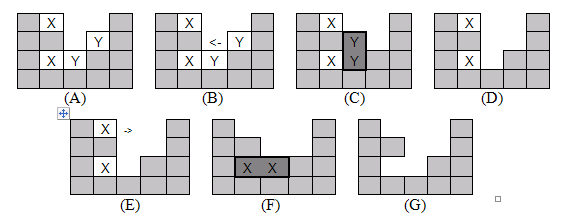
\includegraphics[width=0.7\textwidth]{../latex/img/1011/1011-1.png}
\end{figure}

พิจารณาภาพ (A) หากมีคำสั่งให้ย้ายบล็อก \textbf{(1, 3, L), (0, 1, R)} ตามลำดับ จะได้ผลลัพธ์ดังภาพ (B) ถึง (G) โดยจะได้คะแนนรวม $20$ คะแนน จากการลบบล็อกจำนวน $4$ บล็อกออกไปจากบอร์ด 

\begin{figure}[h]
\centering
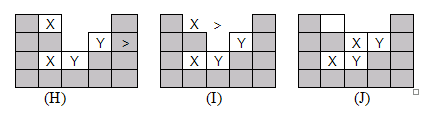
\includegraphics[width=0.7\textwidth]{../latex/img/1011/1011-2.png}
\end{figure}

อย่างไรก็ตาม พิจารณาจากภาพ (A) หากมีคำสั่งให้ย้ายบล็อก \textbf{(1, 3, R), (0, 1, R)} ตามลำดับ จะได้ผลลัพธ์ดังภาพ (H) ถึง (J) ซึ่งไม่สามารถย้ายบล็อกใดๆ ออกไปจากบอร์ดได้ ในกรณีนี้จะได้คะแนนรวม $-5$ คะแนน จากการย้ายบล็อก \textbf{(1, 3, R)} ไปในทิศทางไม่ถูกต้อง (ย้ายบล็อกไปตำแหน่งของบอร์ด) และหลังจากย้ายบล็อก \textbf{(0, 1, R)} ไม่มีบล็อกใดถูกลบออกไปจากบอร์ด

\newpage

รับประกันว่าในข้อมูลทดสอบจะไม่มีกรณีเริ่มต้นที่มีบล็อกชนิดเดียวกันติดกัน และในระหว่างการเคลื่อนย้ายบล็อกจะไม่มีกรณีที่มีกลุ่มของบล็อกชนิดเดียวกันติดกันมากกว่าหนึ่งชุดในเวลาเดียวกัน

(อย่างไรก็ตามหลังจากลบบล็อกออกจากบอร์ดแล้วอาจมีบล็อกชนิดเดียวกันตกลงมาและทำให้ถูกลบออกต่อไปได้)

\underline{\textbf{โจทย์}}  จงเขียนโปรแกรมเพื่อรับข้อมูลโครงสร้างบอร์ดและบล็อก และข้อมูลการเคลื่อนย้ายบล็อก จากนั้นคำนวณหาคะแนนของการย้ายบล็อก พร้อมทั้งแสดงโครงสร้างใหม่ของบอร์ดและบล็อก

\InputFile

\textbf{บรรทัดแรก} มีเลขจำนวนเต็มบวกสองจำนวน $m$ $n$  (แต่ละค่าจะคั่นด้วยช่องว่างหนึ่งช่อง) แทนขนาดของแถว และสดมภ์ของบอร์ดตามลำดับ

\textbf{บรรทัดที่ $2$ ถึง $m+1$} บรรทัดที่ $i+1$ รับข้อมูลโครงสร้างของบอร์ดและบล็อกในแถวที่ $i$ โดยใช้เครื่องหมาย \textbf{“\#”} แทนบอร์ด, \textbf{“-”} แทนพื้นที่ว่าง และอักษรตัวใหญ่แทนชนิดของบล็อก ระหว่างแต่ละสดมภ์จะคั่นด้วยช่องว่างหนึ่งช่อง

\textbf{บรรทัดที่ $m+2$} รับจำนวนเต็มบวก $k$ $(1 \leq k \leq 20)$ แทนจำนวนการเคลื่อนย้ายบล็อก

\textbf{บรรทัดที่ $m+3$ ถึง $m+k+2$} บรรทัดที่ $m+i+2$ เป็นคำสั่งการเคลื่อนย้ายบล็อกลำดับที่ $i$ ซึ่งประกอบด้วยค่า $3$ ค่า แต่ละค่าจะคั่นด้วยช่องว่างหนึ่งช่องดังนี้
\begin{itemize}

\item ค่าแรกเป็นจำนวนเต็ม บอกตำแหน่งแถวจากบนลงล่างเริ่มต้นจากศูนย์
\item ค่าที่สองเป็นจำนวนเต็ม บอกตำแหน่งสดมภ์จากซ้ายไปขวาเริ่มต้นจากศูนย์
\item ค่าที่สามเป็นตัวอักษร บอกทิศทางการเคลื่อนย้าย โดย “L” ไปทางซ้าย และ “R” ไปทางขวา
\end{itemize}

\OutputFile

\textbf{บรรทัดแรก} แสดงจำนวนเต็มหนึ่งจำนวน แทนคะแนนรวมจากการเคลื่อนย้ายบล็อก

\textbf{บรรทัดที่ $2$ ถึง $m+1$} บรรทัดที่ $i+1$  แสดงโครงสร้างใหม่ของบอร์ดและบล็อกในแถวที่ $i$ หลังจากทำการเคลื่อนย้ายตามเงื่อนไขทั้งหมดแล้ว

\Examples

\begin{example}
\exmp{4 5
\# A - - \#
\# \# - B \#
\# A B \# \#
\# \# \# \# \#
2
1 3 L
0 1 R}{20
\# - - - \#
\# \# - - \#
\# - - \# \#
\# \# \# \# \#}%
\exmp{5 5
\# A – B \#
\# B - A \#
\# \# - B \#
\# A B \# \#
\# \# \# \# \#
3
0 1 L
0 3 L
0 1 R}{20
\# - - - \#
\# B - - \#
\# \# - A \#
\# - - \# \#
\# \# \# \# \#}%
\end{example}

\Source

การแข่งขันคอมพิวเตอร์โอลิมปิก สอวน. ครั้งที่ 3 มหาวิทยาลัยขอนแก่น

\end{problem}

\end{document}